%%%%%%%%%%%%%%%%%%%%%%%%%%%%%%%%%%%%%%%%%
% Arsclassica Article
% LaTeX Template
% Version 1.1 (1/8/17)
%
% This template has been downloaded from:
% http://www.LaTeXTemplates.com
%
% Original author:
% Lorenzo Pantieri (http://www.lorenzopantieri.net) with extensive modifications by:
% Vel (vel@latextemplates.com)
%
% License:
% CC BY-NC-SA 3.0 (http://creativecommons.org/licenses/by-nc-sa/3.0/)
%
%%%%%%%%%%%%%%%%%%%%%%%%%%%%%%%%%%%%%%%%%

%----------------------------------------------------------------------------------------
%	PACKAGES AND OTHER DOCUMENT CONFIGURATIONS
%----------------------------------------------------------------------------------------

\documentclass[
12pt, % Main document font size
a4paper, % Paper type, use 'letterpaper' for US Letter paper
oneside, % One page layout (no page indentation)
headinclude,footinclude, % Extra spacing for the header and footer
BCOR5mm, % Binding correction
german]{scrartcl}


\usepackage[onehalfspacing]{setspace}
\usepackage{mathtools}
\usepackage[export]{adjustbox}
\usepackage{babel,varioref}
\addto\extrasgerman{% page 5 of varioref's manual
  \renewcommand\reftextfaceafter{auf der n{\"a}chsten Seite}%
  \renewcommand\reftextafter {auf der n{\"a}chsten Seite}%
  \renewcommand\reftextfacebefore{auf der vorherigen Seite}%
  \renewcommand\reftextbefore {auf der vorherigen Seite}%
  \renewcommand\reftextcurrent {auf dieser Seite}%
}

%%%%%%%%%%%%%%%%%%%%%%%%%%%%%%%%%%%%%%%%%
% Arsclassica Article
% Structure Specification File
%
% This file has been downloaded from:
% http://www.LaTeXTemplates.com
%
% Original author:
% Lorenzo Pantieri (http://www.lorenzopantieri.net) with extensive modifications by:
% Vel (vel@latextemplates.com)
%
% License:
% CC BY-NC-SA 3.0 (http://creativecommons.org/licenses/by-nc-sa/3.0/)
%
%%%%%%%%%%%%%%%%%%%%%%%%%%%%%%%%%%%%%%%%%

%----------------------------------------------------------------------------------------
%	REQUIRED PACKAGES
%----------------------------------------------------------------------------------------

\usepackage[
nochapters, % Turn off chapters since this is an article        
beramono, % Use the Bera Mono font for monospaced text (\texttt)
eulermath,% Use the Euler font for mathematics
pdfspacing, % Makes use of pdftex’ letter spacing capabilities via the microtype package
dottedtoc % Dotted lines leading to the page numbers in the table of contents
]{classicthesis} % The layout is based on the Classic Thesis style

\usepackage{arsclassica} % Modifies the Classic Thesis package

\usepackage[T1]{fontenc} % Use 8-bit encoding that has 256 glyphs

\usepackage[utf8]{inputenc} % Required for including letters with accents

\usepackage{graphicx} % Required for including images
\graphicspath{{Figures/}} % Set the default folder for images

\usepackage{enumitem} % Required for manipulating the whitespace between and within lists

\usepackage{lipsum} % Used for inserting dummy 'Lorem ipsum' text into the template

\usepackage{subcaption} % Required for creating figures with multiple parts (subfigures)

\usepackage{amsmath,amssymb,amsthm} % For including math equations, theorems, symbols, etc

%\usepackage{varioref} % More descriptive referencing

%----------------------------------------------------------------------------------------
%	THEOREM STYLES
%---------------------------------------------------------------------------------------

\theoremstyle{definition} % Define theorem styles here based on the definition style (used for definitions and examples)
\newtheorem{definition}{Definition}

\theoremstyle{plain} % Define theorem styles here based on the plain style (used for theorems, lemmas, propositions)
\newtheorem{theorem}{Theorem}

\theoremstyle{remark} % Define theorem styles here based on the remark style (used for remarks and notes)

%----------------------------------------------------------------------------------------
%	HYPERLINKS
%---------------------------------------------------------------------------------------

\hypersetup{
%draft, % Uncomment to remove all links (useful for printing in black and white)
colorlinks=true, breaklinks=true, bookmarks=true,bookmarksnumbered,
urlcolor=webbrown, linkcolor=RoyalBlue, citecolor=webgreen, % Link colors
pdftitle={}, % PDF title
pdfauthor={\textcopyright}, % PDF Author
pdfsubject={}, % PDF Subject
pdfkeywords={}, % PDF Keywords
pdfcreator={pdfLaTeX}, % PDF Creator
pdfproducer={LaTeX with hyperref and ClassicThesis} % PDF producer
} % Include the structure.tex file which specified the document structure and layout

\hyphenation{Fortran hy-phen-ation} % Specify custom hyphenation points in words with dashes where you would like hyphenation to occur, or alternatively, don't put any dashes in a word to stop hyphenation altogether

%----------------------------------------------------------------------------------------
%	TITLE AND AUTHOR(S)
%----------------------------------------------------------------------------------------

\title{\normalfont\spacedallcaps{Image deobfuscation of Gaussian Blur and Mosaic}} % The article title

%\subtitle{Subtitle} % Uncomment to display a subtitle
\author{Antonio Galeazzi (inf102867@fh-wedel.de) \\ und \\ Till Hildebrandt (inf102835@fh-wedel.de)}

\date{} % An optional date to appear under the author(s)

%----------------------------------------------------------------------------------------

\begin{document}
%----------------------------------------------------------------------------------------
%	HEADERS
%----------------------------------------------------------------------------------------

\renewcommand{\sectionmark}[1]{\markright{\spacedlowsmallcaps{#1}}} % The header for all pages (oneside) or for even pages (twoside)
\lehead{\mbox{\llap{\small\thepage\kern1em\color{halfgray} \vline}\color{halfgray}\hspace{0.5em}\rightmark\hfil}} % The header style

\pagestyle{scrheadings} % Enable the headers specified in this block

\captionsetup[figure]{labelfont={bf},name={Abbildung}}
\newcommand\amusingversion[2]{%
    \vrefpagenum\firstnum{#1}%
    \vrefpagenum\secondnum{#2}%
    \ifthenelse{\equal\firstnum\secondnum}%
    {s of \ref{#1} and \ref{#2} \vpageref{#1}}%
    { of \ref{#1} \vpageref{#1} and of \ref{#2} \vpageref{#2}}%
    }


%----------------------------------------------------------------------------------------
%	TABLE OF CONTENTS & LISTS OF FIGURES AND TABLES
%----------------------------------------------------------------------------------------

\maketitle % Print the title/author/date block

\setcounter{tocdepth}{2} % Set the depth of the table of contents to show sections and subsections only

\tableofcontents % Print the table of contents

\listoffigures % Print the list of figures

\listoftables % Print the list of tables

%----------------------------------------------------------------------------------------
%	ABSTRACT
%----------------------------------------------------------------------------------------

\section*{Abstract} % This section will not appear in the table of contents due to the star (\section*)

Diese Arbeit setzt sich mit der Verwendung von Convolutional Neuroal Networks (CNNs) zum Wiederherstellen
unkenntlich gemachter Gesichtsbilder (engl. face obfuscated) auseinander. Ziel ist es ein CNN aufzubauen,
welches ein mögliches Urspurngsbild zu einem eingegebenen verfälschten Bild liefert.



%----------------------------------------------------------------------------------------

\newpage % Start the article content on the second page, remove this if you have a longer abstract that goes onto the second page

%----------------------------------------------------------------------------------------
%	INTRODUCTION
%----------------------------------------------------------------------------------------

\section{Einleitung}
%\renewcommand{\thefootnote}{\arabic{footnote}}

In bildgebenden Medien, Videos wie Fotos, werden Gesichter von Menschen verfälscht, um deren Identität unkenntlich
zu machen.\footnote{Andrew Senior, Protecting Privacy in Video Surveillance, S 130 ff.\label{label:protecting_privacy}}
Diese Technologien werden von
öffentlichen Medien, wie Privatpersonen verwendet. In der Vergangenheit
gab es den Fall eines Kinderschänders, der verfälschte Gesichtsbilder von sich veröffentlichte. Er verwendete dabei
ein Verfahren, das Pixel um einen zentralen Punkt zu einer Spirale rotiert. Behörden war es damals möglich, diese
Form der Gesichtsverfälschung, der Informationsverlust im Vergleich zu den Verfahren, die in dieser Arbeit behandelt
werden, gering ist, aufzuheben und das Gesicht weitgehends wiederherzustellen.
\footnote{Vancouver Sun, "Convicted 'swirl face' sex offender Christopher Neil to live in Vancouver".
(http://vancouversun.com/news/local-news/convicted-swirl-face-sex-offender-christopher-neil-to-live-in-vancouver)},
\footnote{Wikipedia, "Christopher Paul Neil". (https://en.wikipedia.org/wiki/Christopher\_Paul\_Neil)}
Motiviert unter anderem dadurch,
stellt diese Arbeit eine Grundlagenanalyse dar, in wie weit CNNs dafür verwendet werden können sehr viel verbreitetere,
aber destruktive Obfuscation-Verfahren anzugreifen.

Maßgablich kommen beim Verfälschen zwei Verfahren zum Einsatz\textsuperscript{\ref{label:protecting_privacy}}:
"Weichzeichnen" (Gaussian Blur),\footnote{Wikipedia, Gaussian Blur. (https://en.wikipedia.org/wiki/Gaussian\_blur)}
und "Verpixelung" (Pixelization)\footnote{Wikipedia, Pixelization. (https://en.wikipedia.org/wiki/Pixelization)\label{label:pixelization}}.


\subsection{Weichzeichnen}
Der gaußscher Weichzeichner oder Gaussian smoothing, beschreibt ein Verfahren, mit dem der Kontrast von Bildern
verrinngert wird. Damit wird der Verlust von Detailinformationen erreicht. Die mathematische Formel, nach der die
Transformation funktioniert, lautet:

\parskip\baselineskip
\(G(x) = \frac{1}{\sqrt{2 \pi \sigma^2}} e^{-\frac{x^2}{2 \sigma^2}}\)
\par
\par

x und y beschreiben die Distanz zum Ursprung der jeweiligen Achse, \(\sigma\) ist ein Parameter der Funktion, der
beschreibt wie sehr die Weichzeichnung streut (siehe Abbildung  \vref*{fig:gaussianBlur}).
Der Formel kann man entnehmen, dass die
Farbinformationen benachbarter Pixel in das Ergebnis des aktuell zu berechnenden Pixels miteinfließen. Hier werden
die Informationen verschiedener Pixel auf den selben Wertebereich eines Pixels abgebildet. Der dadurch entstehende
Informationsverlust ist irreversibel.

\begin{figure}[h]
    \centering
    \begin{subfigure}{0.3\textwidth}
        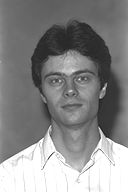
\includegraphics[width=0.9\textwidth]{introduction_blur_original}
        \caption{Original}
    \end{subfigure}
    \begin{subfigure}{0.3\textwidth}
        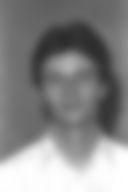
\includegraphics[width=0.9\textwidth]{introduction_blur_sigma_3}
        \caption{\(\sigma = 3\)}
    \end{subfigure}
    \begin{subfigure}{0.3\textwidth}
        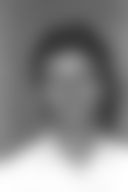
\includegraphics[width=0.9\textwidth]{introduction_blur_sigma_6}
        \caption{\(\sigma = 6\)}
    \end{subfigure}

    \caption{Vergleichsbild Weichzeichnen mit verschiedenen Parametern.}
    \label{fig:gaussianBlur}
\end{figure}

\subsection{Verpixelung}
Auch Mosaic-Verfahren, meint eine Menge an Verfahren, die die Auflösung von Bildern oder Bereiche derer künstlich
verringern, um Detailinformationen zu verbergen. Hierfür wird der unkenntlich zu machende Bereich in gleichmäßige
Unterbereiche aufgeteilt und deren resultierender Farbwert aus den Pixeln des Ursprungsbildes gemittelt. Bei dieser
Verfahrensfamilie gibt es eine Vielzahl an Variationen, die sich in Größe und Form der Unterbereiche und dem genauen
Algorithmus, der verwendet wird, um die Unterbereiche unkenntlich zu machen. \ref{label:pixelization}

\begin{figure}[h]
    \centering
    \begin{subfigure}{0.3\textwidth}
        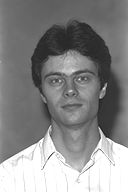
\includegraphics[width=0.9\textwidth]{introduction_mosaic_original}
        \caption{Original}
    \end{subfigure}
    \begin{subfigure}{0.3\textwidth}
        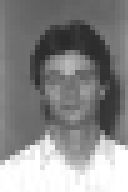
\includegraphics[width=0.9\textwidth]{introduction_mosaic_5}
        \caption{Kantenlänge 5px}
    \end{subfigure}
    \begin{subfigure}{0.3\textwidth}
        
\includegraphics[width=0.9\textwidth]{introduction_mosaic_10}
        \caption{Kantenlänge 10px}
    \end{subfigure}

    \caption{Vergleichsbild Weichzeichnen mit verschiedenen Kantenlängen.}
    \label{fig:pixelization}
\end{figure}

Der in diesem Verfahren betrachtete Parameter (siehe Abbildung  \vref*{fig:pixelization}) entspricht der Kantenlänge der resultierenden verpixelten Unterbereiche.





%------------------------------------------------

\subsection{Paragraphs}

\lipsum[6] % Dummy text

\paragraph{Paragraph Description} \lipsum[7] % Dummy text

\paragraph{Different Paragraph Description} \lipsum[8] % Dummy text

%------------------------------------------------

\subsection{Math}

\lipsum[4] % Dummy text

\begin{equation}
\cos^3 \theta =\frac{1}{4}\cos\theta+\frac{3}{4}\cos 3\theta
\label{eq:refname2}
\end{equation}

\lipsum[5] % Dummy text

\begin{definition}[Gauss] 
To a mathematician it is obvious that
$\int_{-\infty}^{+\infty}
e^{-x^2}\,dx=\sqrt{\pi}$. 
\end{definition} 

\begin{theorem}[Pythagoras]
The square of the hypotenuse (the side opposite the right angle) is equal to the sum of the squares of the other two sides.
\end{theorem}

\begin{proof} 
We have that $\log(1)^2 = 2\log(1)$.
But we also have that $\log(-1)^2=\log(1)=0$.
Then $2\log(-1)=0$, from which the proof.
\end{proof}

%----------------------------------------------------------------------------------------
%	RESULTS AND DISCUSSION
%----------------------------------------------------------------------------------------

\section{Results and Discussion}

Reference to Figure~\vref{fig:gallery}. % The \vref command specifies the location of the reference

\begin{figure}[tb]
\centering 
\includegraphics[width=0.5\columnwidth]{GalleriaStampe} 
\caption[An example of a floating figure]{An example of a floating figure (a reproduction from the \emph{Gallery of prints}, M.~Escher,\index{Escher, M.~C.} from \url{http://www.mcescher.com/}).} % The text in the square bracket is the caption for the list of figures while the text in the curly brackets is the figure caption
\label{fig:gallery} 
\end{figure}

\lipsum[10] % Dummy text

%------------------------------------------------

\subsection{Subsection}

\lipsum[11] % Dummy text

\subsubsection{Subsubsection}

\lipsum[12] % Dummy text

\begin{description}
\item[Word] Definition
\item[Concept] Explanation
\item[Idea] Text
\end{description}

\lipsum[12] % Dummy text

\begin{itemize}[noitemsep] % [noitemsep] removes whitespace between the items for a compact look
\item First item in a list
\item Second item in a list
\item Third item in a list
\end{itemize}

\subsubsection{Table}

\lipsum[13] % Dummy text

\begin{table}[hbt]
\caption{Table of Grades}
\centering
\begin{tabular}{llr}
\toprule
\multicolumn{2}{c}{Name} \\
\cmidrule(r){1-2}
First name & Last Name & Grade \\
\midrule
John & Doe & $7.5$ \\
Richard & Miles & $2$ \\
\bottomrule
\end{tabular}
\label{tab:label}
\end{table}

Reference to Table~\vref{tab:label}. % The \vref command specifies the location of the reference

%------------------------------------------------

\subsection{Figure Composed of Subfigures}

Reference the figure composed of multiple subfigures as Figure~\vref{fig:esempio}. Reference one of the subfigures as Figure~\vref{fig:ipsum}. % The \vref command specifies the location of the reference

\lipsum[15-18] % Dummy text

\begin{figure}[tb]
\centering
%\subfloat[A city market.]{\includegraphics[width=.45\columnwidth]{Lorem}} \quad
%\subfloat[Forest landscape.]{\includegraphics[width=.45\columnwidth]{Ipsum}\label{fig:ipsum}} \\
%\subfloat[Mountain landscape.]{\includegraphics[width=.45\columnwidth]{Dolor}} \quad
%\subfloat[A tile decoration.]{\includegraphics[width=.45\columnwidth]{Sit}}
\caption[A number of pictures.]{A number of pictures with no common theme.} % The text in the square bracket is the caption for the list of figures while the text in the curly brackets is the figure caption
\label{fig:esempio}
\end{figure}

%----------------------------------------------------------------------------------------
%	BIBLIOGRAPHY
%----------------------------------------------------------------------------------------

\renewcommand{\refname}{\spacedlowsmallcaps{References}} % For modifying the bibliography heading

\bibliographystyle{unsrt}

\bibliography{sample.bib} % The file containing the bibliography

%----------------------------------------------------------------------------------------

\end{document}